\section{Results}
\label{sec:results}

\subsection{Week 2: Static Environment}

The static evaluation used 40 paired start-goal scenarios on a 15$\times$15 grid with obstacle density 0.20 and seed 42. Start-goal pairs were drawn from the free cells of a single \texttt{GridEnvironment} instance and validated against Dijkstra on that same grid. The DQN evaluation environment had the same 15$\times$15 obstacle layout as the Dijkstra environment, achieved by directly copying \texttt{simra\_env.blocked} into the DQN grid after construction; this is a stronger guarantee than matching seeds, as it carries no dependency on RNG implementation details agreeing between the two environment classes. Dijkstra computed a single shortest-path query per scenario; the DQN policy ran a full episode from each start to goal.

\begin{table}[h]
\centering
\caption{Static Evaluation Summary (40 scenarios). Compute-time figures were re-measured for this revision on the evaluation machine used throughout this paper; they are of the same order as, but not numerically identical to, the originally reported figures, consistent with the hardware sensitivity noted in Sec.~\ref{sec:compute-time-measurement}.}
\resizebox{\columnwidth}{!}{%
\begin{tabular}{lcc}
\toprule
Metric & Dijkstra & DQN \\
\midrule
Success rate & 40/40 (100\%) & 39/40 (97.5\%) \\
Mean path cost & --- & +0.9248 above Dijkstra \\
Max suboptimality gap & --- & +3.6569 \\
Mean compute time (all scenarios) & 0.72 ms & 3.86 ms \\
Mean compute time (successes only) & 0.72 ms & 2.40 ms \\
\bottomrule
\end{tabular}%
}
\label{tab:static-summary}
\end{table}

DQN matched Dijkstra exactly (gap = 0) on 14 of 39 successful scenarios and produced a higher path cost on the remaining 25. The single failure (start $(12,0)$, goal $(13,10)$) was a step-limit timeout at 225 steps with no collision, indicating the policy entered a loop rather than crashing. The compute-time figures are route-level totals as defined in Section~\ref{sec:compute-time-measurement}: one Dijkstra call per scenario versus accumulated \texttt{.predict()} calls per DQN episode. Both the success/path-cost figures and the compute-time figures in Table~\ref{tab:static-summary} were produced by an independent re-run of the static evaluation for this revision (Sec.~\ref{sec:experimental-setup}); the success-rate and path-cost numbers matched the original run exactly, which is expected since both Dijkstra and the loaded DQN checkpoint are deterministic at evaluation time (\texttt{deterministic=True} action selection), while the compute-time numbers were newly measured rather than reused. On this re-run, DQN was on average $3.3\times$ slower than Dijkstra on scenarios where DQN succeeded, and $5.4\times$ slower when the one timeout episode --- which pays the full 225-step budget of forward passes before terminating --- is included.

\subsection{Dynamic Environment}
\label{sec:dynamic-results}

The dynamic evaluation used 50 paired start-goal scenarios sharing the same scenario IDs and start-goal pairs across all three methods. Static obstacle density was set to 0.0 on all sides; the only changing cells were the three shared dynamic obstacles at $(4,4)$, $(8,8)$, and $(12,11)$, each toggling on a five-step period. Dijkstra and A* both succeeded in all 50 scenarios; the RL policy succeeded in 49 of 50. The failed RL scenario is included in success-rate reporting but excluded from paired path-cost and compute-time statistics because no valid RL path cost exists for it, leaving $n=49$ scenarios where all three methods succeeded for the paired comparisons below.

\subsubsection{Success Rate}

Figure~\ref{fig:success-rate} shows the success rate for Dijkstra and RL as originally reported. Table~\ref{tab:success-ci} adds A* and reports 95\% Wilson confidence intervals for all three methods given the small sample size. Dijkstra and A* both achieved 100\% success (50/50); RL achieved 98\% (49/50). The confidence intervals overlap substantially at this sample size --- with only 50 trials, a single-scenario difference in outcome is not enough to separate 100\% from 98\% with strong confidence on its own. The success-rate comparison should therefore be read alongside the path-cost comparison below, where the sample is larger in effect (49 paired, non-tied observations) and the statistical evidence is much stronger.

\begin{table}[h]
\centering
\caption{Dynamic-evaluation success rate with 95\% Wilson confidence intervals (50 scenarios each).}
\begin{tabular}{lcc}
\toprule
Method & Success rate & 95\% Wilson CI \\
\midrule
Dijkstra & 50/50 (100.0\%) & [92.9\%, 100.0\%] \\
A* & 50/50 (100.0\%) & [92.9\%, 100.0\%] \\
RL (DQN+HER) & 49/50 (98.0\%) & [89.5\%, 99.6\%] \\
\bottomrule
\end{tabular}
\label{tab:success-ci}
\end{table}

\begin{figure}[t]
    \centering
    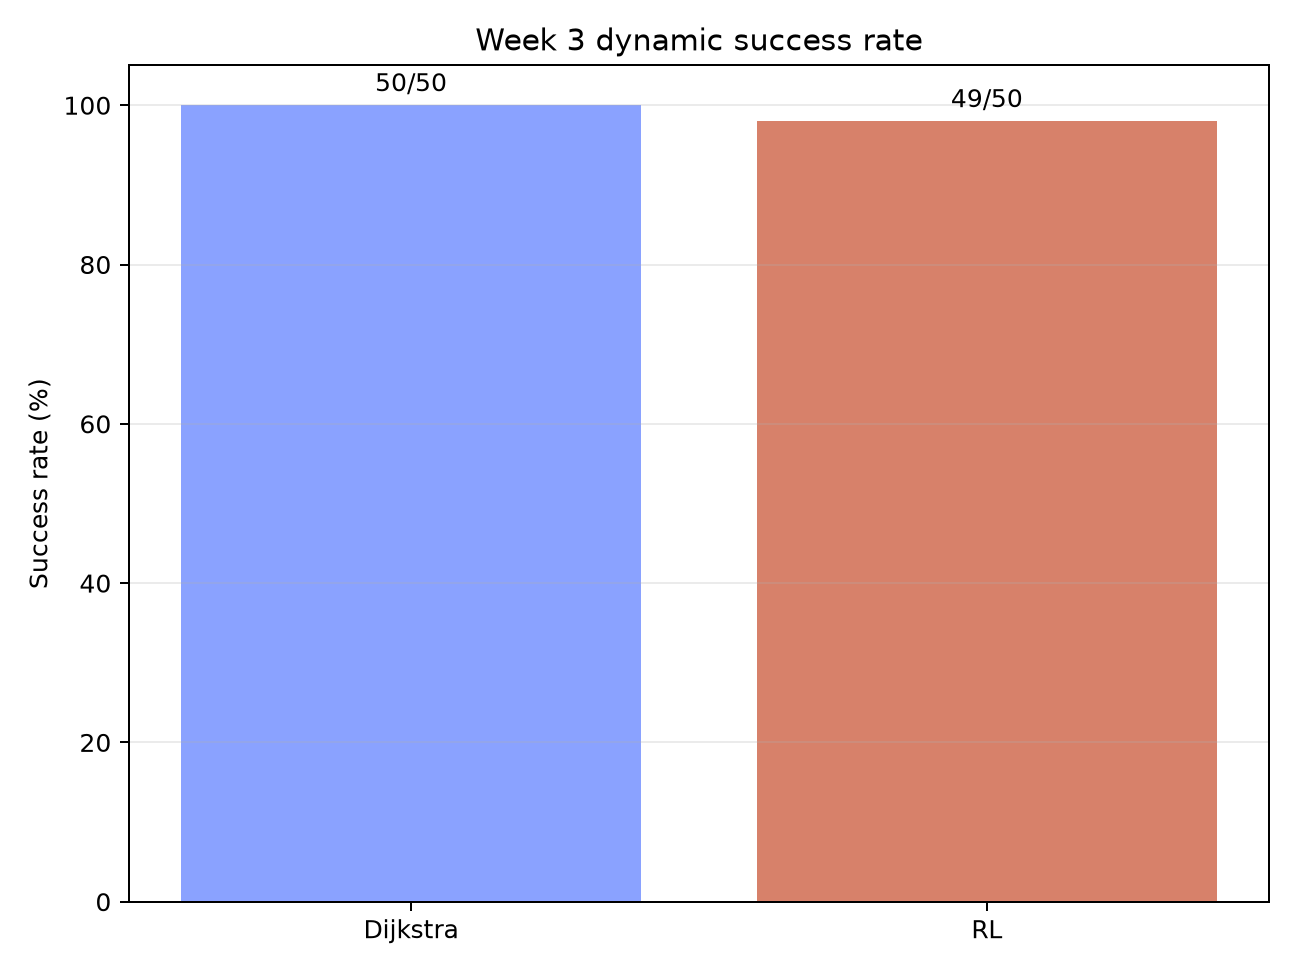
\includegraphics[width=0.9\linewidth]{figures/week4_success_rate.png}
    \caption{Dynamic-routing success rate over 50 matched scenarios.}
    \label{fig:success-rate}
\end{figure}

\subsubsection{Path Cost}

Path-cost statistics are computed on the 49 scenarios where both methods succeeded. Dijkstra was never more expensive than RL: RL matched Dijkstra in 16 scenarios and produced a higher path cost in 33 scenarios. The mean path-cost difference, measured as RL minus Dijkstra, was +1.369441, and the median difference was +0.828427.

\begin{figure}[t]
    \centering
    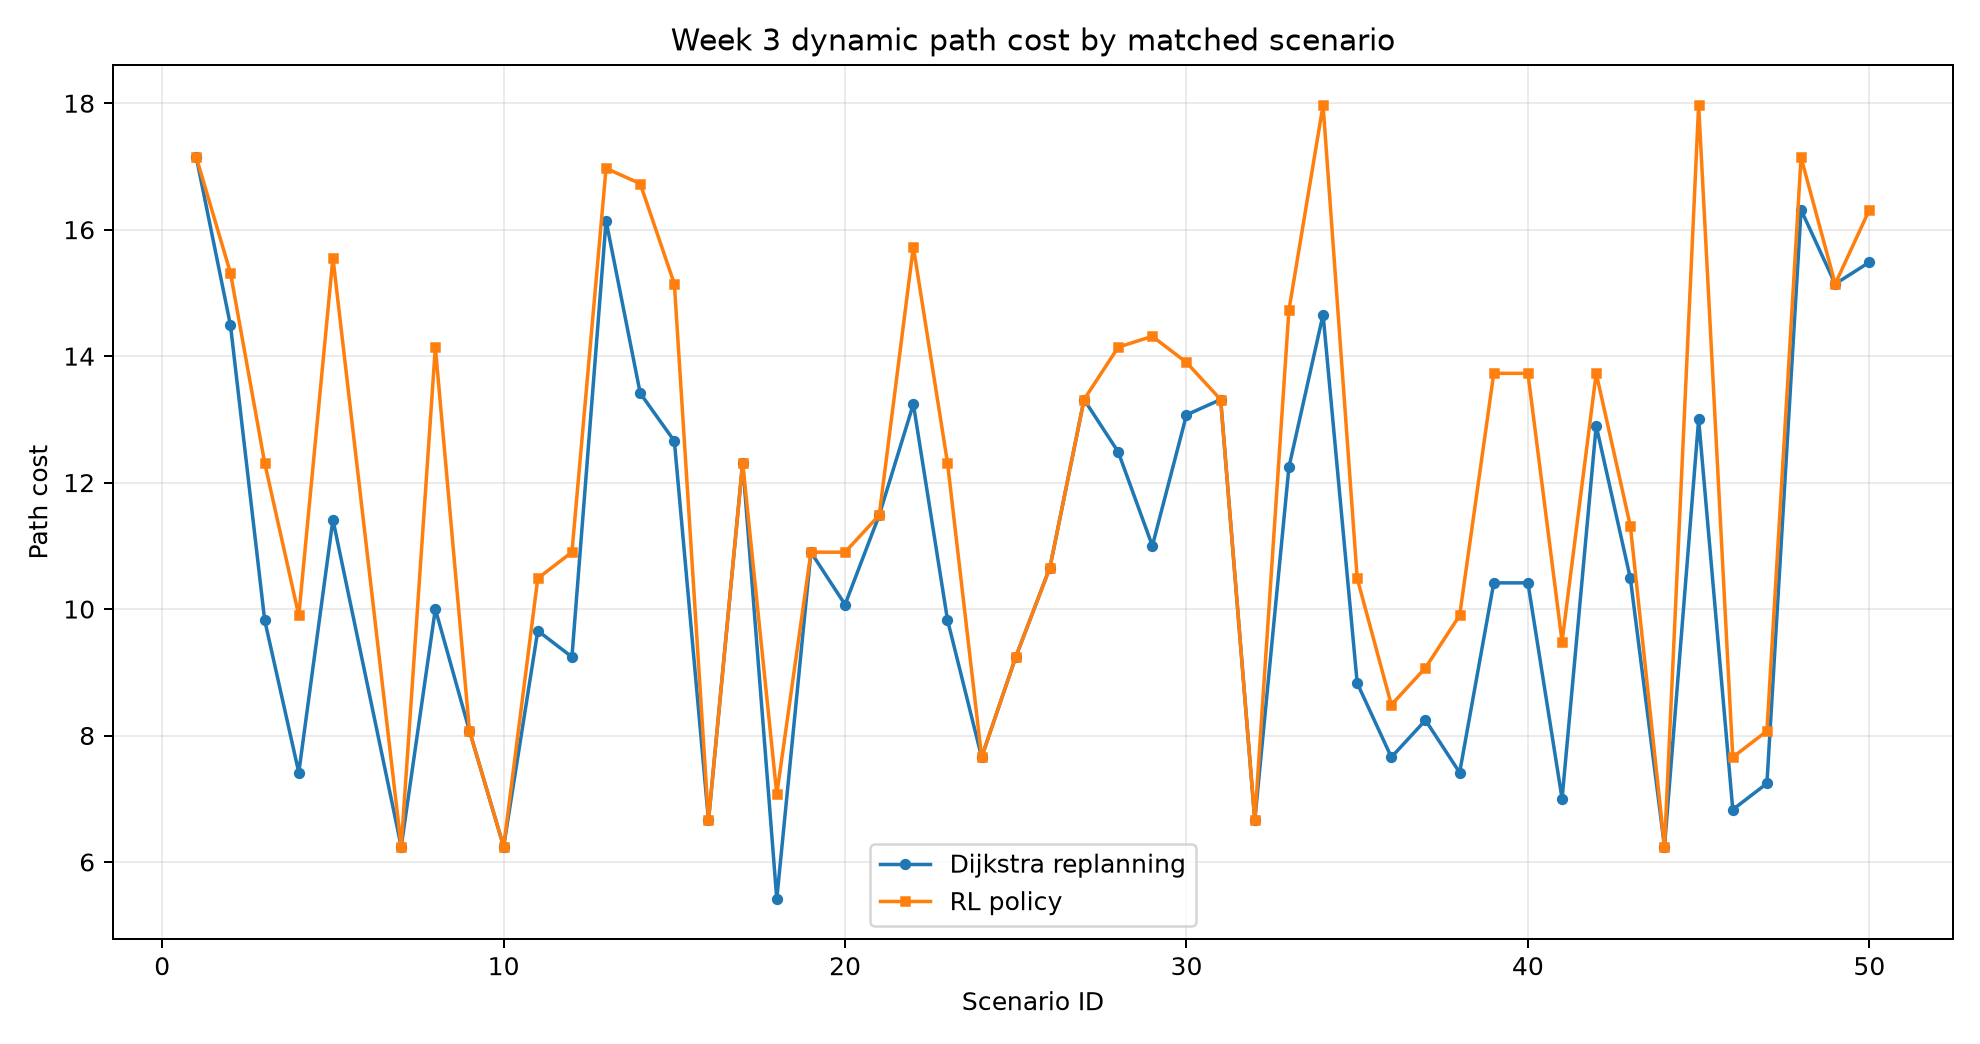
\includegraphics[width=\linewidth]{figures/week4_path_cost_comparison.png}
    \caption{Dynamic path cost by matched scenario for Dijkstra replanning and RL.}
    \label{fig:path-cost-comparison}
\end{figure}

\begin{figure}[t]
    \centering
    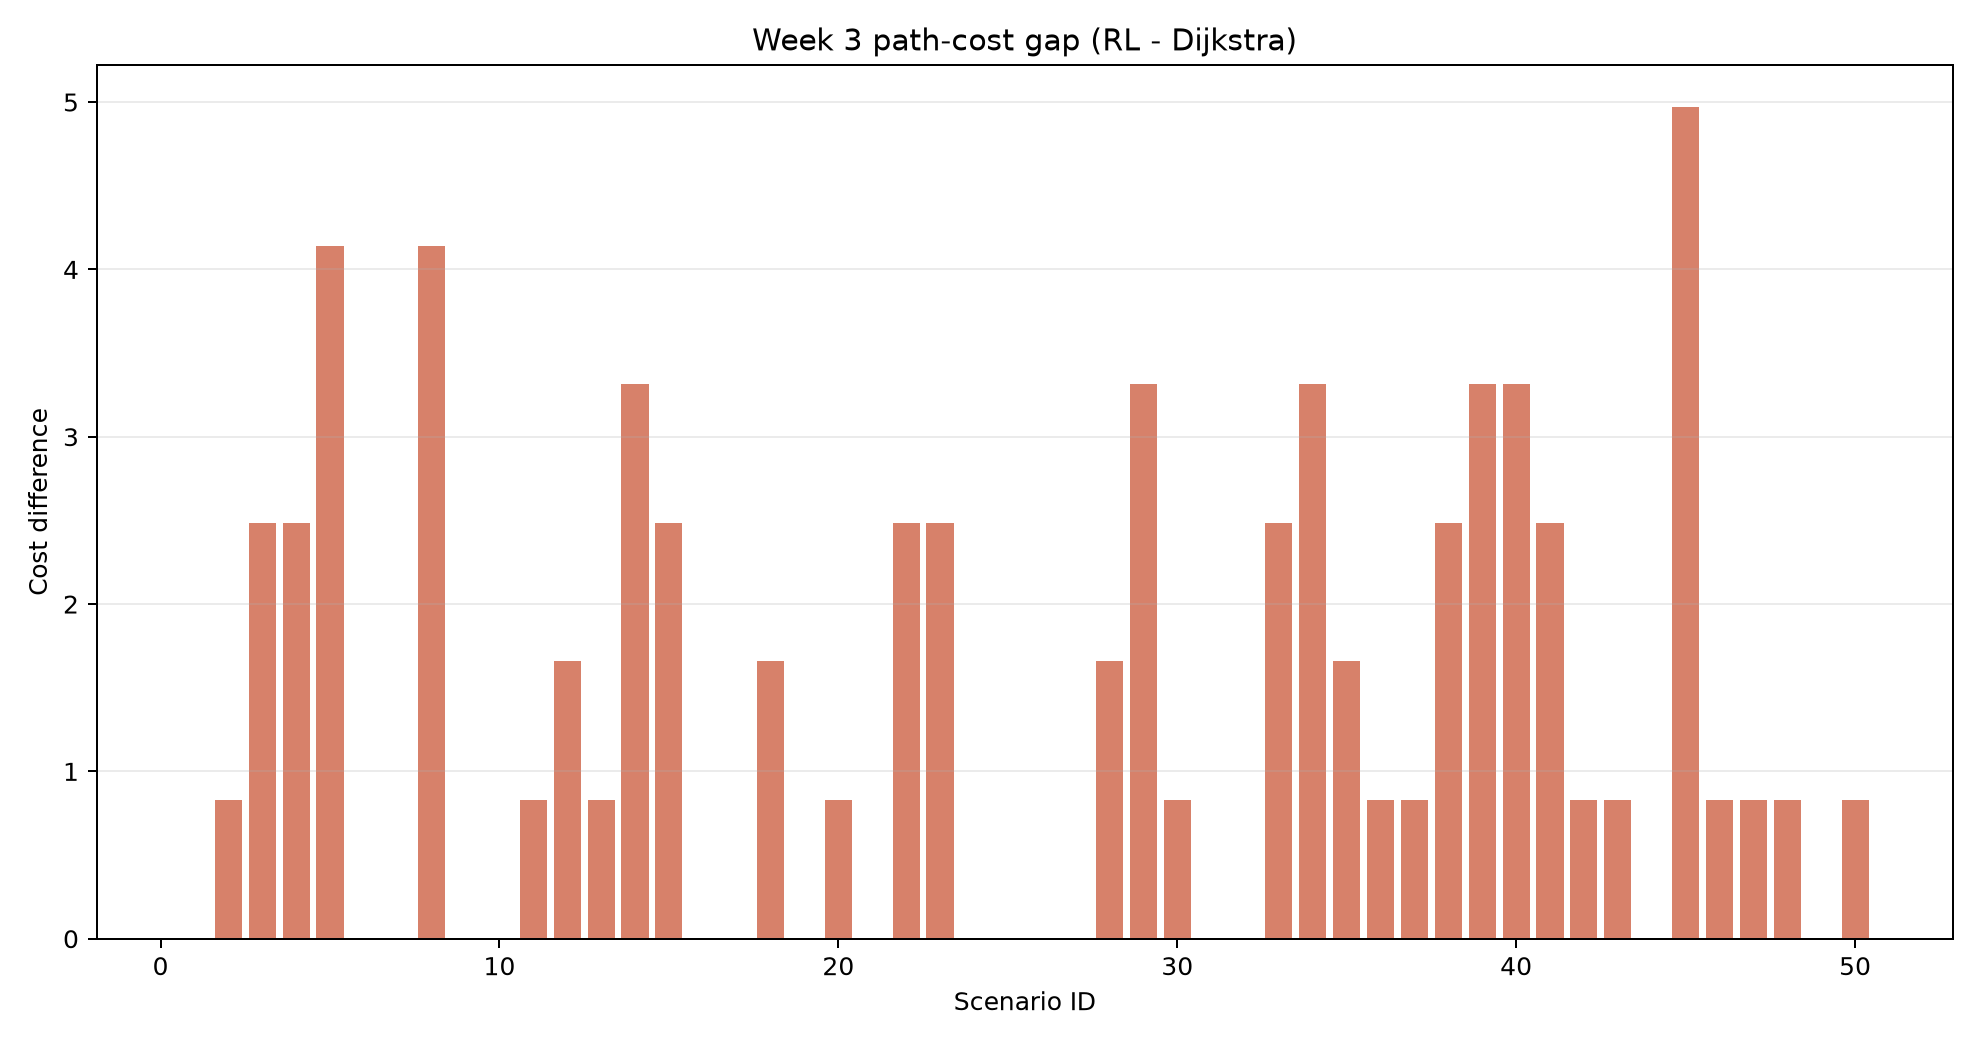
\includegraphics[width=\linewidth]{figures/week4_path_cost_gap.png}
    \caption{Path-cost gap measured as RL minus Dijkstra. Positive values indicate higher RL path cost.}
    \label{fig:path-cost-gap}
\end{figure}

A Wilcoxon signed-rank test on paired path-cost differences gave $W=0$ and $p=5.64\times10^{-7}$. This result is statistically significant, indicating that Dijkstra produced significantly shorter or equal paths than RL in the tested dynamic environment.

Because A* is optimal on this non-negative-weight graph, its dynamic path cost was identical to Dijkstra's on all 49 jointly-successful scenarios (mean and maximum absolute difference both $0.000000$), exactly as predicted by the algorithms' shared optimality guarantee. Consequently RL's path-cost gap against A* is numerically identical to its gap against Dijkstra (Wilcoxon $W=0$, $p=5.23\times10^{-7}$, computed independently on the A*-paired subset). This identity is itself a useful sanity check: it confirms that A* was implemented and evaluated correctly against the same graph and edge costs as Dijkstra, and that the RL policy's cost disadvantage is a genuine gap against \emph{optimal} planning, not an artifact of which classical planner happens to be used as the reference.

\subsubsection{Compute Time}

Mean cumulative Dijkstra planning time was 4.628 ms, while mean RL evaluation time was 5.334 ms on the paired successful scenarios ($n=49$). The Wilcoxon p-value for this compute-time difference was 0.063, which is not statistically significant at $p<0.05$ --- the finding reported in the original evaluation.

\begin{figure}[t]
    \centering
    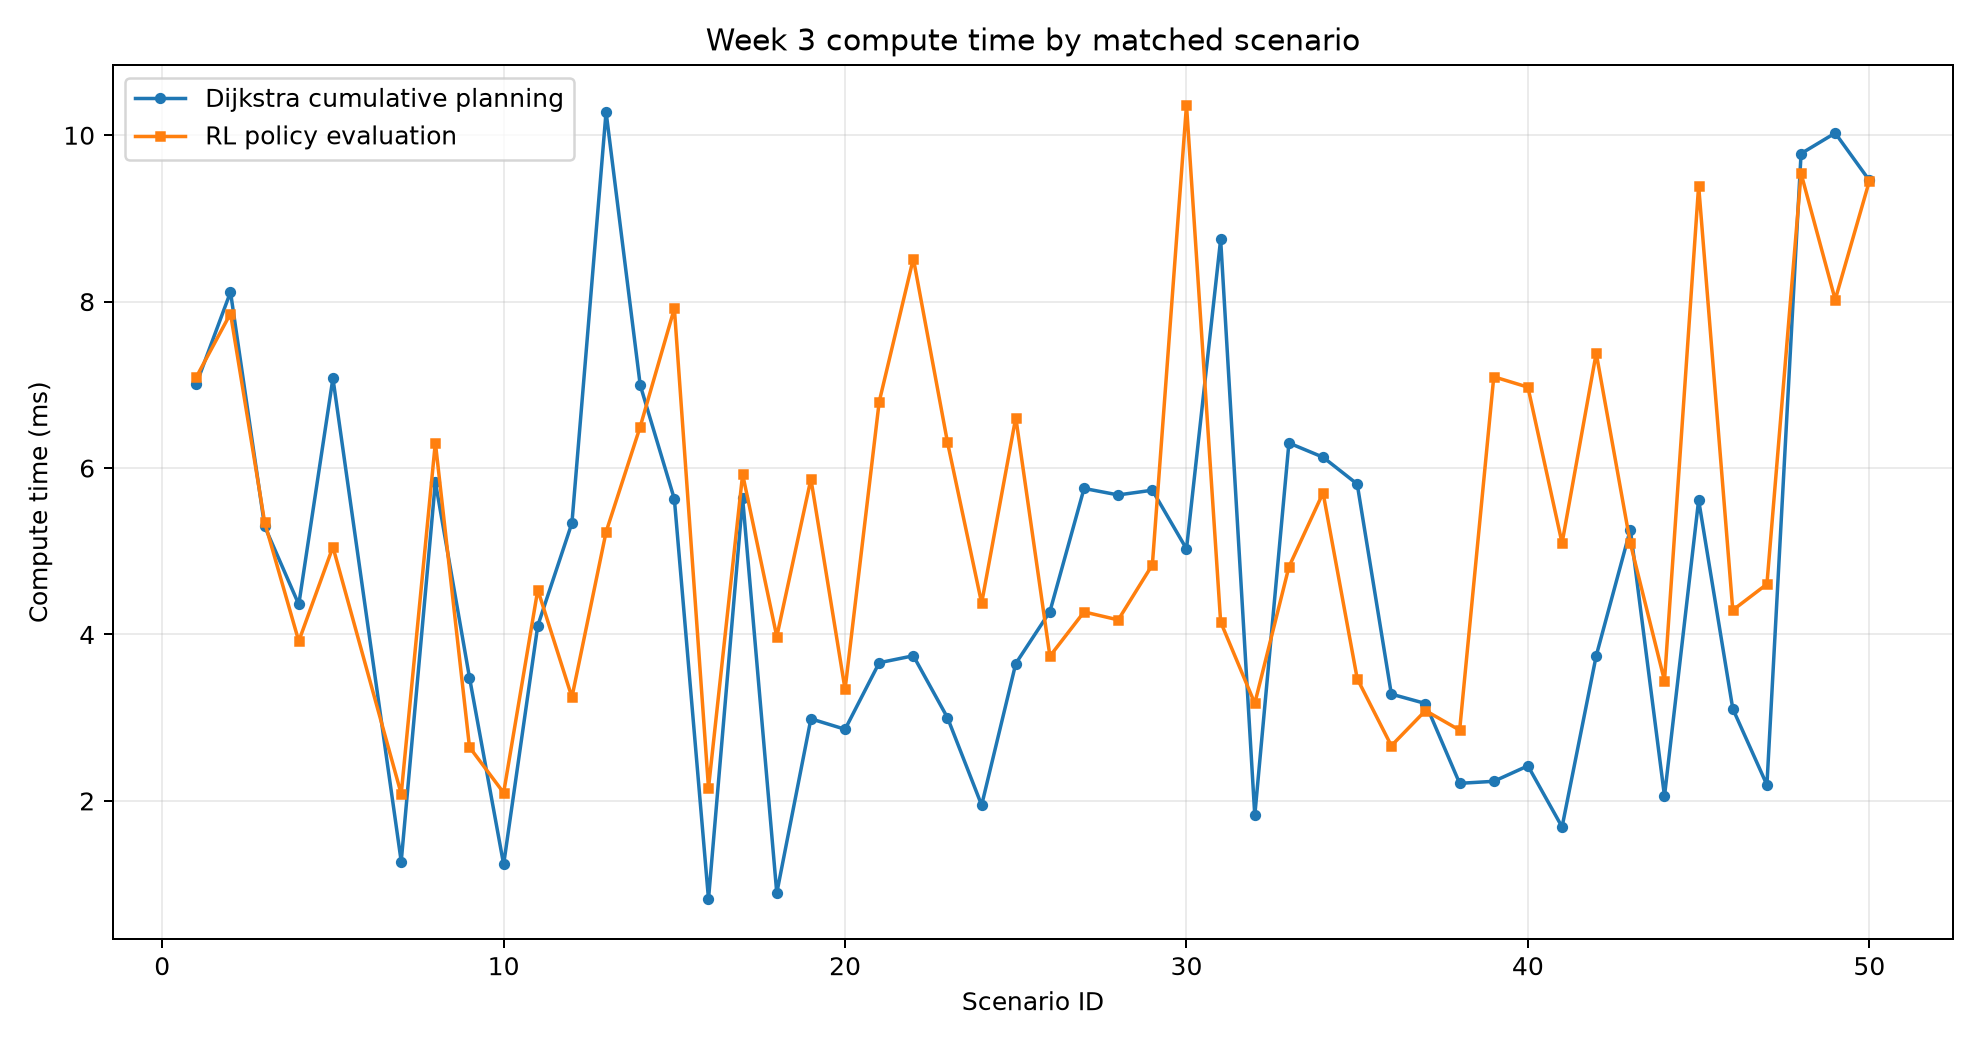
\includegraphics[width=\linewidth]{figures/week4_compute_time_comparison.png}
    \caption{Compute time by matched scenario. Dijkstra time is cumulative replanning time; RL time is policy evaluation time.}
    \label{fig:compute-time}
\end{figure}

Adding A* changes this picture substantially. A* resolved the same replanning events --- an identical mean of 2.45 replans per scenario, since both classical planners react to the same dynamic-obstacle triggers --- in a mean of 0.288 ms, versus Dijkstra's 4.628 ms: roughly \textbf{16$\times$ faster}, driven by A*'s heuristic pruning reducing mean node expansions per scenario to 31.7 out of the grid's 225 cells, compared to Dijkstra's exhaustive expansion. A paired Wilcoxon test on A* vs.\ Dijkstra compute time gives $p=3.6\times10^{-15}$, and A* vs.\ RL compute time gives the same order of significance ($p=3.6\times10^{-15}$, A* faster). Figure~\ref{fig:astar-compute-time} places all three methods on the same axis.

\begin{figure}[t]
    \centering
    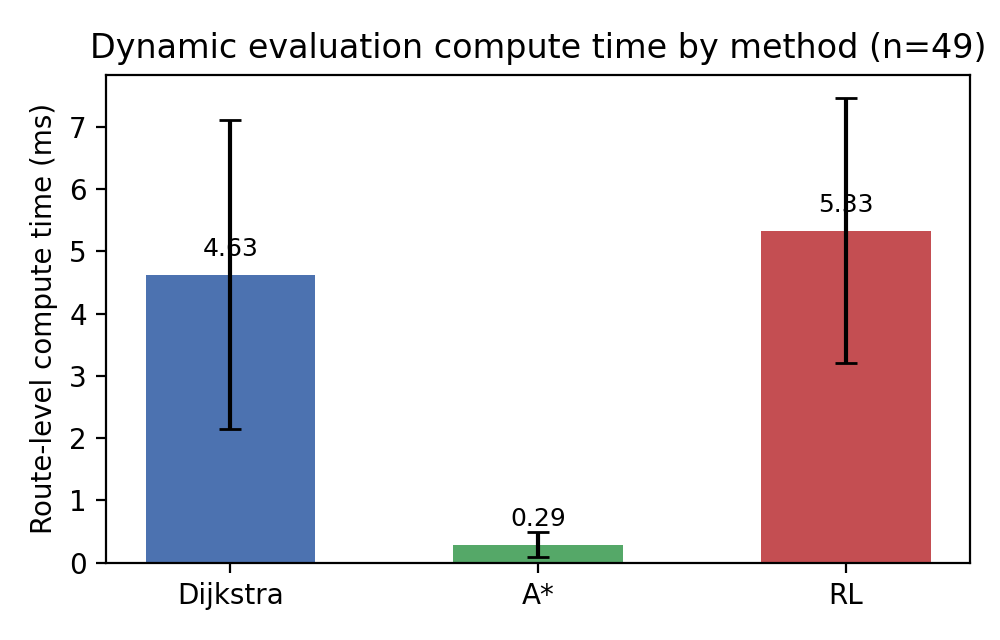
\includegraphics[width=0.95\linewidth]{figures/week5_astar_compute_time.png}
    \caption{Mean route-level compute time by method on the 49 jointly-successful dynamic scenarios (error bars: 1 std.\ dev.). A* resolves the same replanning events as Dijkstra roughly 16$\times$ faster at identical path cost.}
    \label{fig:astar-compute-time}
\end{figure}

This reframes the original compute-time conclusion. The original paper's non-significant $p=0.063$ result compared RL only against \emph{naive} Dijkstra and concluded that ``the anticipated compute-time advantage of RL did not reach significance... likely because the grid is small enough that repeated Dijkstra replanning remains cheap.'' That explanation undersold the classical side: a large part of naive Dijkstra's cost is not an inherent property of graph-search replanning at this grid size, but a consequence of not pruning the search at all. Once a standard, easy-to-implement heuristic is added, the classical planner becomes decisively faster than both naive Dijkstra \emph{and} RL, while still returning optimal paths. RL's per-step forward-pass cost, which the original discussion framed as a potential deployment-time advantage over repeated graph search, does not materialize as an advantage against either classical baseline at this grid size --- it is the slowest of the three methods in route-level compute time.

\subsection{Generalization Probe}
\label{sec:generalization}

The evaluations above all use the same fixed grid layout (seed 42) that the RL policy was trained on, since \texttt{fixed\_grid=True} was used throughout training to make HER's reward computation tractable (Sec.~\ref{sec:rl-policy}). This means the reported RL success rates describe performance on a grid the policy has effectively memorized the structure of, not generalization to unseen layouts. As an informal robustness probe conducted during development, the Phase-3 checkpoint was additionally evaluated on 50 episodes drawn from a single unseen obstacle layout (seed 999, not used anywhere in training or in the reported evaluations), with random start/goal pairs rather than the fixed 50-scenario protocol used elsewhere in this paper. The agent reached the goal in 47 of 50 episodes (94\%), with zero collisions and three step-limit timeouts. Trace inspection of the three timeouts showed the agent navigating correctly for most of each episode before entering a two-cell oscillation after being structurally cut off from a direct route by an obstacle configuration not present in the training grid; reward magnitudes during these episodes were small and correctly scaled ($-0.02$ to $-0.17$ per step), which rules out the earlier Q-value overestimation bug (Sec.~\ref{sec:rl-policy}) as the cause and points instead to a pure generalization gap from single-layout training.

We report this result as a directional signal, not a rigorous generalization benchmark: it uses one unseen seed rather than a distribution of layouts, was not paired against Dijkstra or A* on the same seed, and predates some of the reward-shaping changes reflected in Table~\ref{tab:hyperparams}. We include it because it is the only evidence in this project bearing on out-of-distribution behavior, and because the failure mode it surfaces --- confident local navigation followed by oscillation rather than exploratory replanning when structurally blocked --- is a more informative limitation than a bare success-rate number would be. A rigorous multi-layout generalization benchmark, ideally with \texttt{fixed\_grid=False} training as already scoped in the project's internal notes, is future work (Sec.~\ref{sec:limitations}).
